% Derived From ACM's "SIGPROC-SP.TEX - VERSION 3.1"

%\nonstopmode
\documentclass{acm_proc_article-sp}
\usepackage{color, soul}
\usepackage{paralist}
\usepackage{algpseudocode}
\usepackage{algorithm,algorithmicx}
\usepackage{listings}
\usepackage{booktabs}

\newcommand{\ttt}[1]{\texttt{#1}}
\DeclareMathOperator{\bigO}{\mathcal{O}}
\def\reals{\mathbb{R}}

\renewcommand{\algorithmicrequire}{\textbf{Input:}}
\renewcommand{\algorithmicensure}{\textbf{Output:}}

\def\a{\mathbf{a}}
\def\u{\mathbf{u}}
\def\v{\mathbf{v}}

\begin{document}

\title{Low-rank Matrix Factorization in Spark\\ on High Performance and Cluster Computing Systems\\ for Scalable and Interpretable Data Analysis}

% Original comment from ACM template:
%
%    You need the command \numberofauthors to handle the 'placement
%    and alignment' of the authors beneath the title.
%   
%    For aesthetic reasons, we recommend 'three authors at a time'
%    i.e. three 'name/affiliation blocks' be placed beneath the title.
%   
%    NOTE: You are NOT restricted in how many 'rows' of
%    "name/affiliations" may appear. We just ask that you restrict
%    the number of 'columns' to three.
%   
%    Because of the available 'opening page real-estate'
%    we ask you to refrain from putting more than six authors
%    (two rows with three columns) beneath the article title.
%    More than six makes the first-page appear very cluttered indeed.
%   
%    Use the \alignauthor commands to handle the names
%    and affiliations for an 'aesthetic maximum' of six authors.
%    Add names, affiliations, addresses for
%    the seventh etc. author(s) as the argument for the
%    \additionalauthors command.
%    These 'additional authors' will be output/set for you
%    without further effort on your part as the last section in
%    the body of your article BEFORE References or any Appendices.
%
% NOTE: This is not the true number of authors, but is a hack based on the
% above comment to compress layout of the authors list and save space.
\numberofauthors{6}

\author{
\alignauthor
Jey Kottalam\\
%%LONG%% \affaddr{Berkeley Institute for Data Science and EECS Department, University of California, Berkeley}\\
\affaddr{BIDS and EECS, UC Berkeley}\\
\email{jey@berkeley.edu}
\alignauthor
Jiyan Yang\\
%%LONG%% \affaddr{Institute for Computational and Mathematical Engineering, Stanford University}\\
\affaddr{ICME, Stanford University}\\
\email{jiyan@stanford.edu}
\alignauthor
Michael F. Ringenberg\\
%%LONG%% \affaddr{Cray Inc}\\
\affaddr{Cray Inc}\\
\email{mikeri@cray.com}
\and
\alignauthor
Jatin Chhugani\\
\email{jatinch@gmail.com}
\alignauthor
Evan Racah\\
%%LONG%% \affaddr{National Energy Research Scientific Computing Division, Lawrence Berkeley National Laboratory}\\
\affaddr{NERSC, LBNL}\\
\email{eracah@lbl.gov}
\alignauthor
Alex Gittens\\
%%LONG%% \affaddr{International Computer Science Institute and Department of Statistics, University of California, Berkeley}\\
\affaddr{ICSI \& Statistics, UC Berkeley}\\
\email{gittens@icsi.berkeley.edu}
\and
\alignauthor
Mohitdeep Singh\\
%%LONG%% \affaddr{Georgia Institute of Technology}\\
\affaddr{Georgia Inst. of Technology}\\
\email{msingh74@gatech.edu}
\alignauthor
Monte LaBute\\
%%LONG%% \affaddr{Cray Inc}\\
\affaddr{Cray Inc}\\
\email{mlabute@cray.com}
\alignauthor
Yushu Yao\\
%%LONG%% \affaddr{National Energy Research Scientific Computing Division, Lawrence Berkeley National Laboratory}\\
\affaddr{NERSC, LBNL}\\
\email{yyao@lbl.gov}
\and
\alignauthor
Curt R. Fischer\\
%%LONG%% \affaddr{Life Sciences Division, Lawrence Berkeley National Laboratory}\\
\affaddr{LSD, LBNL}\\
\email{crfischer@lbl.gov}
\alignauthor
Oliver Ruebel\\
%%LONG%% \affaddr{Computational Research Division, Lawrence Berkeley National Laboratory}\\
\affaddr{CRD, LBNL}\\
\email{oruebel@lbl.gov}
\alignauthor
Benjamin P. Bowen\\
%%LONG%% \affaddr{Life Sciences Division, Lawrence Berkeley National Laboratory}\\
\affaddr{LSD, LBNL}\\
\email{bpbowen@lbl.gov}
\and
\alignauthor
Michael W. Mahoney\\
%%LONG%% \affaddr{International Computer Science Institute and Department of Statistics, University of California, Berkeley}\\
\affaddr{ICSI \& Statistics, UC Berkeley}\\
\email{mmahoney@stat.berkeley.edu}
\alignauthor
Venkat Krishnamurthy\\
%%LONG%% \affaddr{Cray Inc}\\
\affaddr{Cray Inc}\\
\email{venkat@cray.com}
\alignauthor
Prabhat\\
%%LONG%% \affaddr{National Energy Research Scientific Computing Division, Lawrence Berkeley National Laboratory}\\
\affaddr{NERSC, LBNL}\\
\email{prabhat@lbl.gov}
}

\maketitle
\begin{abstract}
\section{Abstract}
\textit{Owners: Jey, Jiyan, Jatin, Prabhat (0.4 pages)}

\end{abstract}

% A category with the (minimum) three required fields
%% TODO FIXME: No idea if this is correct. -JK
\category{H.2.8}{Database Management}{Database Applications}
%\category{C.4}{ PERFORMANCE OF SYSTEMS }{}
%\category{G.4}{ MATHEMATICAL SOFTWARE }{}

%% TODO: what keywords should we use? -JK
\keywords{ACM proceedings, \LaTeX, text tagging} % NOT required for Proceedings

\section{Introduction}
\label{sec:intro}

Matrix algorithms are increasingly important in many large-scale data analysis applications.  
Essentially, the reason is that matrices (i.e., sets of vectors in Euclidean spaces) provide a convenient mathematical structure with which to model data arising in a broad range of applications:
an $m \times n$ real-valued matrix $A$ provides a natural structure for
encoding information about $m$ objects, each of which is described by $n$
features;
alternatively, an $n \times n$ real-values matrix $A$ can be used to describe
the correlations between all pairs of $n$ data points, or the weighted
edge-edge adjacency matrix structure of an $n$-node graph.%
\footnote{For example, in astronomy, small angular regions of the sky imaged at a range of electromagnetic frequency bands can be represented as a matrix, where an object is a region and the features are the elements of the frequency bands;
in genetics, DNA SNP (Single Nucleotide Polymorphism) or DNA microarray expression data can be represented in such a framework, with $A_{ij}$ representing the expression level of the $i^{th}$ gene or SNP in the $j^{th}$ experimental condition or individual; and
in many Internet and social media applications, term-document matrices can be constructed, with $A_{ij}$ indicating the frequency of the $j^{th}$ term in the $i^{th}$ document.}
Importantly, the data model and natural operations associated with matrices and vector spaces (i.e., scalar multiplication and vector addition) are much more sophisticated than the data model and natural operations (e.g., selects, joins, etc.) associated with traditional flat tables.

In particular, the low-rank approximation to a data matrix $A$ that is provided by performing a truncated SVD (singular value decomposition)---or PCA (principal component analysis) or CX/CUR decompositions---is a very complicated object---both conceptually and computationally---compared with what is conveniently supported by traditional database operations~\cite{Skillicorn07}.
Recall that PCA is a popular method that finds the mutually orthogonal eigencomponents that maximize the variance captured by the factorization, and CX/CUR provides an interpretable low-rank factorization by selecting a small number of columns/rows from the original data matrix as its factors.
Described in more detail in Section \ref{sxn:low-rank-methods}, these low-rank approximation methods are popular in small- and medium-scale machine learning and scientific data analysis applications for exploratory and interactive data analysis and for providing compact and/or interpretable representations of complex matrix-based data, but their implementation at scale remains a challenge.

Relatedly, the computation of quantities like eigenvectors, eigenvalues, invariant subspaces, etc., often requires complex communication patterns, with sophisticated iterative techniques that pay careful attention to numerical contitioning issues.
Existing linear algebra code (e.g., LAPACK) is typically develiped for single machines, and effort is typically devoted to minimizing the number of FLOPS (floating-point operations per second) and to do subspace iteration, Lanczos methods, etc. is involved in terms of linear algebra and communication~\cite{templates}.  
While there has been work on minimizing communication in linear algebra algorithms~\cite{BJHS11} as well as some very large-scale HPC (high-performance computing) implementations of algorithms for common matrix problems~\cite{XXX-WHAT-IS-A-GOOD-HPC-LA-REF-HERE}, these are often specialized and require control over processors and communication, e.g., with MPI (message passing interface), thus hindering their broader applicability in many large-scale machine learning and data analysis pipelines.


In particular, these methods do not mesh well with much of the work that has been popular recently in large scale data analysis.
For example, MapReduce/Hadoop does such and such reading and writing at every step and thus iterative algorithms are prohibitive~\cite{DG08_CACM}. 
Apache SPark solves some of these problems by maintiaing some additional state, but even there systems are not designed for nontrivial matrix algorithms~\cite{SPARK_NSDI_12}.
LA methods that ahve been applied are typically PageRank, which are basically trivial from an LA perspective.

In this paper, we report our results on the performance, scalability, and applicability of several related randomized low-rank matrix approximation algorithms in a particular representative scientific application using a popular computational framework on both high-performance and cluster computing systems.
Before providing a summary of our results, we would like to describe in more detail the motivation for the setup for our computations.
\begin{compactitem}
\item
Randomized PCA and randomized CX/CUR low-rank matrix factorizations. 
Randomization, e.g., random sampling and random projection, has proven to be a powerful computational resource for the development of improved linear algebra algorithms, both in worst-case theory and in high-quality numerical implementations~\cite{Mah-mat-rev_BOOK}; and recent results have shown that these algorithms can be implemented in parallel and distributed environments~\cite{YMM15_TR}.
\item
On a 1 TB mass spectrometry imaging (MSI) dataset.
MSI provides a real science use case, where the downstream domain scientists are interested in interactivity and interpretation as well as scalability~\cite{YRPMB15}.
This is a very different set of metrics that performing slightly better on a precision-recall metric, as is more common in typical machine learning workflows.
In addition, this particular dataset is taken from OpenMSI~\cite{OpenMIS13}, A CLOUD COMPUTING THING THAT HAS DATA STORED AT LBL.
\item
Using Apache Spark. 
This has proven to be a popular framework that addresses several of the deficiencies of MapReduce/Hadoop for very large-scale data computations, e.g., iterative computations and interactive analytics, that are particularly important for linear algebra computations.
XXX.  JEY COMMENT.
\item
On an Amazon EC2 cluster, a Cray XC30, and an experimental Cray cluster.  
While most of the work on Spark has focused on cluster computing systems, most of the work in scientific computing and large-scale linear algebra has focused on high-performance systems, and it is of interest to understand how matrix computations perform on high-performance systems when implemented in the Spark system.
XXX.  SOMEONE COMMENT.
\end{compactitem}

Here are our main results.
XXX.  SHOULD THIS BE BEFORE OR AFTER THE ABOVE SET OF BULLETS.
\begin{compactitem}
\item
XXX.
\item
XXX.
\item
XXX.
\item
We have evaluated the scaling properties in both these distributed and parallel environments for these matrix computations, and we have confirmed that we can provide PCA-based as well as interpretable CX/CUR low-rank approximation results to mass spectrometry scientists at much larger size scales than previously possible.  
\end{compactitem}

XXX.  ARCHITECTURAL TRENDS.

%% Some things:
%% 
%% HPC versus distributed data center
%% 
%% High precision versus low-precision
%% 
%% Scientific applications versus Internet applications
%%
%%Interpretable and interactive analytics

Here are some things to include:
\begin{itemize}

\item include discussion about what CX solves and why should the community care about it? <Michael Mahoney>  XXX.  MM TO DO IN SXN 2.

\item How can database community benefit from CX? <??>  XXX.  MM TO DO IN SXN 2.

\item Applicability to various domains. <Michael Mahoney>  XXX.  MM TO DO IN SXN 2 AND HERE.

\item word on increasing dataset sizes (nnzs -- $10^{12}$?)  <Michael, Jey, Prabhat>

 \item Why HPC problem? Why should be fast?

\item Why focusing on SPARK? and not on any other platform? <Jey>

\item Architecture trend... Increasing SIMD width, number of cores, etc. Memory bandwidth not increasing at the same rate. Imp. to devise algorithms that block for caches and thereby compute vs bandwidth bound <Jatin, Mike R.>
    
\end{itemize}


XXX.  MWM TO INCORPORATE THIS PAR INTO SECTION TWO WHEN HE MAKES THE PASS OVER IT.
Recent work in Randomized Linear Algebra (RLA) has focused on using randomization, e.g., random projection and random sampling methods, to perform scalable linear albegra computations~\cite{Mah-mat-rev_BOOK}.
In addition to doing PCA/SVD/LS at scale, work in LRA has focused on so-called CX/CUR decompositions~\cite{DMM08,CUR_PNAS}; these are low-rank matrix decompositions that are expressed in terms of a small number of columns/rows, i.e, actual data elements, and not a small number of eigencolumns/eigenrows.
As such, they have found applicability in many scientific applications where coupling analytical techniques with domain knowleges is at a premium, including genetics~\cite{Paschou07b}, astronomy~\cite{Yip14-AJ}, and mass spectrometry imaging~\cite{YRPMB15}.
Here is the Halko review~\cite{HMT09_SIREV}; and here is a review on implementing randomized matrix algorithms in parallel and distributed environments~\cite{YMM15_TR}.




\section{Low-rank matrix factorization methods}
\label{sxn:low-rank-methods}
%% \textit{Owners: Jiyan, Michael Mahoney (1 page)}

Given an $m \times n$ data matrix $A$, low-rank matrix factorization methods aim find two or more smaller matrices such that their product is a good approximation to $A$.
That is, they aim to find matrices $B$ and $C$ such that
\begin{equation}
 \label{eqn:apprx}
    \underset{m\times n}{A} \approx \underset{m\times k}{Y} \times \underset{k\times n}{Z} , 
\end{equation}
where $Y \times Z$ is a rank-$k$ approximation to the original matrix $A$.
Low-rank matrix factorization methods are an important topic in linear algebra and numerical analysis, and they find use in a variety of scientific fields and scientific computing as well as in machine learning and data analysis applications such as pattern recognition and personalized recommendation.
These methods have the following advantages.
\begin{compactitem}
\item
They are often useful in data compression, as smaller matrices can be stored more efficiently.
\item
In some cases, the results of analysis using them are more interpretable.
For example, in imaging analysis, the original images can be reconstructed using linear combination of basis images.
\item
They can be viewed as a basic dimension reduction technique.
In many modern applications, datasets containing a massive number of rows or columns are becoming more common, which makes it difficult for data visualization or applying classic algorithms, but low-rank approximation methods express every data point in a low-dimensional space defined by only a few features.
\end{compactitem}

Depending on the application, various low-rank factorization techniques are of interest. 
Popular choices include the singular value decomposition~\cite{GVL96}, principal component analysis~\cite{pcaBook}, rank-revealing QR factorization~\cite{GE96}, nonnegative matrix factorization~\cite{NMFalg}, and CUR/CX decomposition~\cite{CUR_PNAS}.
In this work, we consider using PCA and CX decomposition for our scalable and interpretable data analysis; and, in the remainder of the section, we briefly describe these decompositions.
For an arbitrary matrix $A$, denote by $\a_i$ its $i$-th column, $\a^j$ its $j$-th row and $\a_{ij}$ its $(i,j)$-th element. 
Hereby, we assume the data matrix $A$ has size $m$ by $n$ and rank $r$.


\subsection{SVD and PCA}

The singular value decomposition (SVD) is the factorization of matrix $A \in \reals^{m\times n}$ into the product of three matrices $U\Sigma V^T$ where $U \in \reals^{m\times r}$ and $V\in \reals^{r\times n}$ have orthonormal columns and $D\in \reals^{r\times r}$ is a diagonal matrix with positive real entries. 
The columns of $U$ and $V$ are called left and right singular vectors and the diagonal entries of $D$ are called singular values. 
For notation convenience, we assume the singular values are sorted such that $\sigma_1\geq \cdots \geq \sigma_r\geq 0$, and this means that the columns of $U$ and $V$ are sorted by the order given by the singular values.  

%if optimality criterion to choose is the square loss ($\ell_2$ loss)
 
The SVD is of such central interest since it provides the ``best'' low-rank matrix approximation with respect to any unitarily matrix norm.
In particular, the quality of  a low-rank approximation can be measured by a data-dependent loss function $L$. 
A typical choice of $L$ is the squared loss, in which case, we seek to find
\begin{equation}
 \label{eqn:obj}
  \min_{\text{rank}(\tilde A) = k} \| A - \tilde A \|_F,
\end{equation}
where the Frobenius norm $\| \cdot \|_F$ is defined as $\|X\|_F^2 = \sum_{i=1}^m \sum_{j=1}^n X_{ij} $.
For any target rank $k\leq r$, the solution to \eqref{eqn:obj} is given by the truncated SVD, i.e., $A_k = U_k \Sigma_k V_k^T$, where $U_k \in \reals^{m\times k}$ and $V_k\in \reals^{n\times k}$ contain the top $k$ singular vectors, i.e., the first $k$ columns of $U$ and $V$, respectively, and $\Sigma_k\in \reals^{k\times k}$ is a diagonal matrix containing the top-$k$ singular values.

Principal component analysis (PCA) and SVD are closely related.
PCA aims to convert the original features into a set of linearly uncorrelated variables called {\it principal components}.
To be more specific, the first principal component is defined to be the direction along which the highest variance possible among the data points is attained, and each succeeding principal component in turn has the largest variance possible subject to the constraint that it is orthogonal to the preceding principal components.
When low-rank methods are appropriate, the number of principal components needed to preserve most of the information in $A$ is far less than the number of original features, and thus the goal of dimension reduction is achieved.

PCA can be defined mathematically and can be computed via the SVD.
Assuming that matrix $A$ has been preprocessed, i.e., each column of the data matrix $A$ has been centered and has unit variance, then the {\it loading} vectors for PCA are given by top-$k$ singular vectors $V_k$, which transform the original $n$ variables into $k$ new components. 
That is, the top-$k$ principal components are given by 
\begin{equation}
  T_k = A V_k = \begin{pmatrix} \sigma_1 \u_1 & \cdots & \sigma_n \u_n \end{pmatrix}.
\end{equation}
Particularly, the $j$-th principal component of the $i$-th row of $A$ is given by 
$t_{ij} = \a^i \v_j = \sigma_j \u_{ij}$.
% MM: I INLINED THIS EQUATION SINCE IT DOESNT LOOK LIKE IT NEEDS TO BE OUTLINED.
% \begin{equation}
%   t_{ij} = \a^i \v_j = \sigma_j \u_{ij}.
% \end{equation}


\subsection{Randomized SVD}

The computation of the SVD (and thus of PCA for a data matrix $A$) is expensive~\cite{GVL96}.
For example, to compute the truncated SVD with rank $k$ using traditional deterministic methods, the running time complexity is $\bigO(mnk)$, and $\bigO(k)$ passes over the dataset are needed.
This  becomes prohibitively expensive when dealing with datasets of even moderately-large size, e.g., $m = 10^6$, $n = 10^4$ and $k = 20$. 
To address these and related issues, recent work in Randomized Linear Algebra (RLA) has focused on using randomized approximation, e.g., random projection and random sampling methods, to perform scalable linear algebra computations
\footnote{For example, RLA algorithms have led to the best worst-case algorithms for least squares and least absolute deviations regression, they have been implemented to high precision and have been shown to beat LAPACK's direct dense least squares solver on essentially any tall dense matrix; they have been been shown to lead to improved low-rank matrix approximation in scientific computing applications, and they have been shown to have improved statistical properties~\cite{Mah-mat-rev_BOOK}.  Thus, while our focus here is on improved low-rank matrix approximation methods in Spark, we expect that similar improvements can be achieved for other related problems.} for large-scale data problems.
For an overview of the RLA area, see~\cite{Mah-mat-rev_BOOK}; for a review of using RLA methods for low-rank matrix approximation, see~\cite{HMT09_SIREV}; and for a review of the theory underlying implementing RLA methods in parallel/distributed environments, see~\cite{YMM15_TR}.

Here, we will use an algorithm described in Halko et al.~\cite{HMT09_SIREV} which uses a random projection to construct a rank-$k$ approximation to $A$ which approximates $A$ nearly as well as $A_k$ does.
The basis of the approximation is computed based on a smaller matrix after applying a random projection on $A$ that with high probability the range space of $A_k$ is preserved. We refer the readers to \cite{HMT09_SIREV,Mah-mat-rev_BOOK} for more details.
Importantly, the algorithm runs in $\bigO(mn \log k)$ time, and the algorithm needs only a constant number of passes over the data matrix. 
These properties becomes extremely desirable in many large-scale data analytics. 
This algorithm, which we refer to as \textsc{RandomizedSVD}, is summarized in Algorithm~\ref{alg:rsvd}.
(Algorithm~\ref{alg:rsvd} calls \textsc{MultiplyGramian}, which is summarized in Algorithm~\ref{alg:gram}, as well as two algorithms, \textsc{Multiply} and \textsc{ThinSVD}, which are standard in numerical linear algebra~\cite{GVL96}.) 
The running time cost for \textsc{RandomizedSVD} is dominated by the matrix-matrix multiplication, which involve making pass over the entire data matrix, appearing in Step 3 and Step 6 of Algorithm~\ref{alg:rsvd}.
However, these steps can be parallelized, and hence \textsc{RandomizedSVD} is well amenable to distributed computing.%
\footnote{We should mention that Step 3 of Algorithm~\ref{alg:rsvd} involves a dense matrix-matrix multiplication, whereas most RLA algorithms, including the variant of \textsc{RandomizedSVD} in~\cite{HMT09_SIREV} uses an FFT-based random projection in order to obtain a faster asymptotic running time.  While our version incurs more FLOPS, it is more parallelizable and thus more suitable for distributed computational environments.}


\begin{algorithm}[tb]
 \caption{{\sc RandomizedSVD} Algorithm}
  \label{alg:rsvd}
  \begin{algorithmic}[1]
    \Require $A \in \reals^{m\times n}$, \
      number of power iterations $q \ge 1$, \
      and rank $r > 0$, slack $\ell \ge 0$ such that $k=r+\ell \leq \operatorname{rank}(A)$.

    % TODO: domain of each result
    \Ensure $U \Sigma V^T \approx \Call{ThinSVD}{A, r}$.

    \State Initialize $B \in \reals^{n\times k}$ by sampling $B_{ij} \sim \mathcal{N}(0, 1)$.

    \For{$q$ times}
        \State $B \gets \Call{MultiplyGramian}{A, B}$
        \State $(B, \_) \gets \Call{ThinQR}{B}$
    \EndFor

    \State Let $Q$ be the first $r$ columns of $B$.

    \State Let $C = \Call{Multiply}{A, Q}$.

    \State Compute $(U, \Sigma, \tilde V^T) = \Call{ThinSVD}{C}$.

    \State Let $V = Q \tilde V$.
    % alternative that doesn't require knowing the distributivity of transpose but looks silly:
    %\State Let $V^T = \tilde V^T Q^T$.

    \end{algorithmic}
\end{algorithm}

\begin{algorithm}[tb]
  \caption{{\sc MultiplyGramian} Algorithm}
  \label{alg:gram}
  \begin{algorithmic}[1]
    \Require $A \in \reals^{m\times n}$, $B \in \reals^{n\times k}$.
    \Ensure $X = A^T A B$.
    \State Initialize $X = 0$.
    \For{each row $a$ in $A$}
        \State $X \gets X + a a^T B$.
    \EndFor
  \end{algorithmic}
\end{algorithm}


\subsection{CX/CUR decompositions}

In addition to developing improved algorithms for PCA/SVD and related problems, work in RLA has also focused on so-called CX/CUR decompositions~\cite{DMM08,CUR_PNAS}.
As a motivation, observe that principal components are eigenvectors of the Gram matrix $A^TA$, and thus they are linear combinations of up to all of the original variables.
A natural question arises: can we reconstruct the matrix using a small number of actual columns of $A$?

CX/CUR decompositions affirmatively answer this question.
That is, these are low-rank matrix decompositions that are expressed in terms of a small number of columns/rows, i.e, actual data elements, and not a small number of eigencolumns/eigenrows (which form the principal components).
As such, they have found applicability in many scientific applications where coupling analytical techniques with domain knowleges is at a premium, including genetics~\cite{Paschou07b}, astronomy~\cite{Yip14-AJ}, and mass spectrometry imaging~\cite{YRPMB15}.

In more detail,
CX decomposition factorizes an $m \times n$ matrix $A$ into two matrices $C$ and $X$, where $C$ is an $m\times c$ matrix that consists of $c$ actual columns
of $A$, and $X$ is a $c \times n$ matrix such that $A\approx CX$.
%That is, linear combinations of the columns of $C$ can recover most of the ``information'' of the matrix $A$.
(CUR decompositions choose $X=UR$, where $R$ is a small number of actual rows of $A$, and $U$ is a low-dimensional encoding matrix~\cite{DMM08,CUR_PNAS}.)
For CX, using the same optimality criterion defined in~\eqref{eqn:obj}, we seek matrices $C$ and $X$ such that the residual error $\|A-CX\|_F$ is small.

The quality of approximation provided by CX/CUR depends on how the columns are chosen.
The algorithm of~\cite{DMM08} that computes a $1\pm\epsilon$ relative-error low-rank CX matrix approximation consists of three basic steps: 
first, compute (either exactly or approximately) the {\it statistical leverage scores} of the columns of $A$;
and second, use those scores as a sampling distribution to select $c$ columns from $A$ and form $C$;
finally once the matrix $C$ is determined, the optimal matrix $X$ with rank-$k$ that minimizes $\|A-CX\|_F$ can be computed accordingly; see~\cite{DMM08} for detailed construction.
The major steps of this \textsc{CXdecomposition}, which uses approximate leverage scores, is provided in Algorithm~\ref{alg:cx}.


 \begin{algorithm}[tb]
 \caption{\textsc{CXDecomposition}}
  \label{alg:cx}
  \begin{algorithmic}[1]
    \Require $A \in \reals^{m\times n}$, rank parameter $k \leq \textrm{rank}(A)$, number of power iterations $q$.

    \Ensure $C$.
    
    %\Function{ColSelect}{$A,k,r$}

    %\State Using algorithm of\cite{DMMW12_JMLR}, compute an approximation of the top-$k$ right singular vectors of $A$ denoted by $\tilde V_k$, using \textsc{RandomizedSVD} with $q$ power iterations.
    \State Compute an approximation of the top-$k$ right singular vectors of $A$ denoted by $\tilde V_k$, using \textsc{RandomizedSVD} with $q$ power iterations.
    
    \State Let $\ell_i = \sum_{j=1}^k \tilde \v_{ij}^2$, where $\tilde \v_{ij}^2$ is the $(i,j)$-th element of $\tilde V_k$, for $i = 1, \ldots, n$. 
    
    \State Define $p_i = \ell_i / \sum_{j=1}^d \ell_j$ for $i=1,\ldots,n$.
    
    \State Randomly sample $c$ columns from $A$ in i.i.d. trials, using the importance sampling distribution $\{p_i\}_{i=1}^n$ .

    %\State \Return The indices with the top $r$ $\ell_i$s.
    
    %\EndFunction

    \end{algorithmic}
\end{algorithm}


Central to the CX decomposition is the underlying sampling distribution, i.e., the leverage scores; and, thus, we now provide some intuition for our choice.
Let $A=U\Sigma V^T$ be the SVD of $A$.
Given a target rank parameter $k$, for $j=1,\ldots,n$, the $j$-th leverage score can be defined as
\begin{equation}
 \label{eqn:lev}
  \ell_j = \sum_{i=1}^k \v_{ji}^2.
\end{equation}
These scores $\{\ell_j\}_{i=1}^{n}$ can be interpreted as how much ``leverage'' or ``influence'' the $j$-th column of $A$ exerts on the best rank-$k$ approximation to $A$. 
As mentioned above, $A_k = \sum_{i=1}^k \sigma_i u_i v_i^T$ gives the best rank-$k$ approximation to $A$.
In fact, $A_k$ can be viewed as the projection of $A$ onto the top-$k$ \emph{left} singular space spanned by the columns of $\begin{pmatrix} u_1 & \cdots & u_k \end{pmatrix}$.
Since multiplying each column by the corresponding singular value does not alter the subspace, we can view
$$
\begin{pmatrix} \sigma_1 u_1 & \cdots & \sigma_k u_k \end{pmatrix}
$$ 
as a basis for this space.  
%Especially, if $A$ has been preprocessed, these vectors are its top-$k$ principal components.
For each column of $A$, we have 
  $$  a_j = \sum_{i=1}^{r} (\sigma_i u_i) v_{ji} \approx \sum_{i=1}^k (\sigma_i u_i) v_{ji}.  $$
That is, the $j$-th column of $A$ can be expressed as a linear combination of the basis of the top-$k$ left singular space with $v_{ji}$ as the coefficients.
%On the other hand, the scores $\{\ell_j\}_{j=1}^{n}$ equal the diagonal elements of the projection matrix onto the top-$k$ \emph{right} singular subspace spanned by $\begin{pmatrix} v_1 & \cdots & v_k \end{pmatrix}$.
%, and thus these statistical leverage scores are a generalization of the diagonal elements of the ``hat matrix'' in regression diagnostics~\cite{MD09}.
For $j=1,\ldots,n$, if we define the {\it normalized leverage scores} as
\begin{equation}
\label{eqn:nlev}
  p_j = \frac{\ell_j}{\sum_{i=1}^n \ell_i},
\end{equation}      
where $\ell_i$ is defined in~\eqref{eqn:lev}, and choose columns from $A$ according to those normalized leverage scores, then (by~\cite{DMM08,CUR_PNAS}) the selected columns are able to reconstruct the matrix $A$ nearly as well as $A_k$ does.

Observe that the running time for \textsc{CXdecomposition} is the computation of the importance sampling distribution.
To compute the leverage scores based on \eqref{eqn:lev}, i.e., exactly, one needs to compute the top $k$ right-singular vectors $V_k$. 
As pointed out above, this is prohibitive data with massive size.
However, just as with our PCA computation, here we can use \textsc{RandomizedSVD} to compute {\it approximate} leverage scores.
This approach, originally proposed by Drineas et al.~\cite{DMMW12_JMLR}, runs in ``random projection time,'' i.e., it requires fewer FLOPS and fewer passes over the data matrix than the traditional deterministic algorithms that compute the leverage scores~exactly.


%Finally, we want to point out that,
%although delivering different low-rank factorizations, both PAC and CX suffer from the fact that they need to truncated SVD.
%To make the algorithms practical on large-scale dataset, one can alleviate the demanding complexity by using randomized SVD. 

%These algorithms compute high-quality approximations to the normalized leverage scores of the input matrix, and the running time of these algorithms depends on the time to apply a random projection to the input matrix, which is much faster than computing the full (or even a truncated) SVD.

\section{Implementation}
\label{sec:implementation}

To support operating on datasets larger than can be stored and processed on a single node,
we implement the algorithms using the Apache Spark cluster computing framework.

\subsection{Spark}
Spark provides a high-level programming model and execution engine for
fault-tolerant parallel and distributed computing, based on a core 
abstraction called a \textit{resilient distributed dataset (RDD)}.
Each RDD may be thought of as a distributed collection of objects that is
partitioned and stored across the Spark cluster.
RDDs are immutable lazily materialized collections supporting functional
programming operations such as \ttt{map}, \ttt{filter}, and \ttt{reduce},
each of which returns a new RDD.
RDDs may be loaded from a distributed file system, computed from other RDDs,
or created by parallelizing a collection within the user's application.
RDDs of key-value pairs may also be treated as associative arrays, with
operations such as \ttt{reduceByKey}, \ttt{join}, and \ttt{cogroup}.
For example, to compute word frequencies of a text dataset in HDFS:
\begin{verbatim}
val dataset: RDD[String] =
      spark.textFile("hdfs://...")

val counts: RDD[(String, Int)] =
      dataset.
      flatMap(line => line.split(" ")).
      map(word => (word, 1)).
      reduceByKey(_ + _)

val countsMap: Map[String, Int] =
      counts.collectAsMap
\end{verbatim}

%%% this para is very incomplete
Spark employs a lazy evaluation strategy for efficiency.
All Spark operations without any immediate side-effects other than returning an RDD are deferred
if possible.
Instead, most operations simply create an entry in the program DAG, recording the input
dependencies and capturing any closures and values needed.
This approach allows Spark to defer computations as much as possible, and when the evaluation
is unavoidable the entire Spark job can be examined by the Scheduler.
This allows the Spark execution engine to batch together related operations, optimize data locality,
and perform more sophisticated scheduling.
A major benefit of Spark over MapReduce is the use of in-memory caching and storage so that data structures
may be reused rather than being recomputed.



\subsection{CX and PCA on Spark}
\label{sec:cx_spark}
The main consideration when implementing CX and PCA in a parallel setting are
efficient implementations of operations involving the data matrix $A$.
All access of $A$ by the CX and PCA algorithms occurs through the
\ttt{RandomizedSVD} routine shared in common.
\ttt{RandomizedSVD} in turn accesses $A$ only through the \ttt{MultiplyGramian} and
\ttt{Multiply} routines, with repeated invocations of \ttt{MultiplyGramian}
accounting for the majority of the algorithm's execution time.

The matrix $A$ is stored as an RDD containing one \ttt{IndexedRow} per row of the input matrix,
where each \ttt{IndexedRow} consists of the row's index and corresponding data vector.
This is a natural storage format for many datasets stored on a distributed or shared file
system, where each row of the matrix is formed from one record of the
input dataset, thereby preserving locality by not requiring data shuffling
during construction of $A$.

We then express \ttt{MultiplyGramian} in a form amenable to efficient distributed implementation
by exploiting the fact that the matrix product $A^TAB$ can be written as a sum of outer products,
as shown in \ref{alg:gram}. This allows for full parallelism across the rows of the matrix with
each row's contribution computed independently, followed by a summation step to accumulate the result.
This approach may be implemented in Spark as a \ttt{map} forming the outer products followed by a \ttt{reduce}
to accumulate the results:
\begin{verbatim}
def multiplyGramian(A: RowMatrix, B: LocalMatrix) =
  A.rows.map(row => row * row.t * B).reduce(_ + _)
\end{verbatim}
This approach forms $2m$ unnecessary temporary matrices of same dimension as the output matrix $n\times k$,
with one per row as the result of the \ttt{map} expression, and the \ttt{reduce} is not done in-place so it
too allocates a new matrix per row.
This results in high GC pressure and makes poor use of the CPU cache, so
we instead remedy this by accumulating the results in-place by replacing the \ttt{map}
and \ttt{reduce} with a single \ttt{treeAggregate}.
The \ttt{treeAggregate} operation is a map-reduce that executes in-place to accumulate the contribution of a 
single worker node, followed by a
tree-structured reduction that efficiently aggregates the results from each worker.
The reduction is performed in multiple stages using a tree topology to avoid creating a single
bottleneck at the driver node to accumulate the results from each worker node.
Each worker emits a relatively large result with dimension $n\times k$, so the
communication savings of having multiple reducer tasks is significant.
\begin{verbatim}
def multiplyGramian(A: RowMatrix, B: LocalMatrix) = {
  A.rows.treeAggregate(LocalMatrix.zeros(n, k))(
    seqOp = (X, row) => X += row * row.t * B,
    combOp = (X, Y) => X += Y
  )
}
\end{verbatim}



\begin{algorithm}[tb]
 \caption{{\sc RandomizedSVD} Algorithm}
  \label{alg:rsvd}
  \begin{algorithmic}[1]
    \Require $A \in \reals^{m\times n}$, \
      number of power iterations $q \ge 1$, \
      and rank $r > 0$, slack $\ell \ge 0$ such that $k=r+\ell \leq \operatorname{rank}(A)$.

    % TODO: domain of each result
    \Ensure $U \Sigma V^T \approx \Call{ThinSVD}{A, r}$.

    \State Initialize $B \in \reals^{n\times k}$ by sampling $B_{ij} \sim \mathcal{N}(0, 1)$.

    \For{$q$ times}
        \State $B \gets \Call{MultiplyGramian}{A, B}$
        \State $(B, \_) \gets \Call{ThinQR}{B}$
    \EndFor

    \State Let $Q$ be the first $r$ columns of $B$.

    \State Let $C = \Call{Multiply}{A, Q}$.

    \State Compute $(U, \Sigma, \tilde V^T) = \Call{ThinSVD}{C}$.

    \State Let $V = Q \tilde V$.
    % alternative that doesn't require knowing the distributivity of transpose but looks silly:
    %\State Let $V^T = \tilde V^T Q^T$.

    \end{algorithmic}
\end{algorithm}

\begin{algorithm}[tb]
  \caption{{\sc MultiplyGramian} Algorithm}
  \label{alg:gram}
  \begin{algorithmic}[1]
    \Require $A \in \reals^{m\times n}$, $B \in \reals^{n\times k}$.
    \Ensure $X = A^T A B$.
    \State Initialize $X = 0$.
    \For{each row $a$ in $A$}
        \State $X \gets X + a a^T B$.
    \EndFor
  \end{algorithmic}
\end{algorithm}

%%%%%%%\begin{itemize}
\textcolor{red}{
\subsection {Platform Used (SPARK) (explain it) }
    \Comment{Jatin}{Jey to explain the SPARK compute node, with some
    details on cache size, cores, SIMD width, etc.}
}

     \begin{figure*}[htp]
         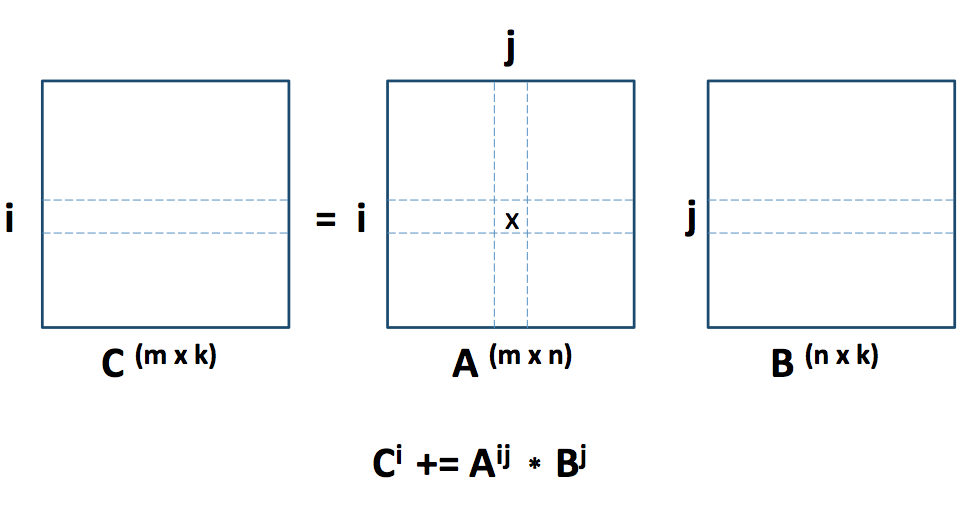
\includegraphics[scale=0.254]{images/jatin_a}
         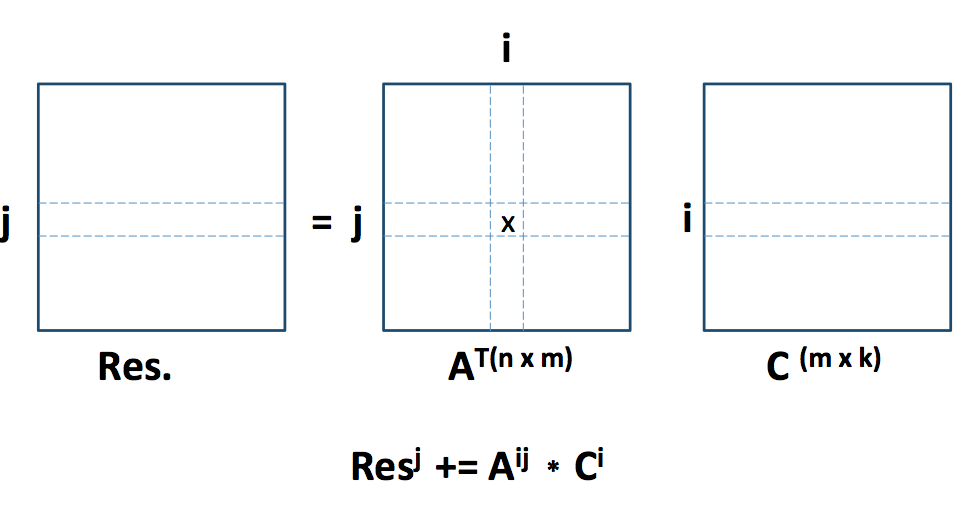
\includegraphics[scale=0.254]{images/jatin_b}
         \caption{ Data access pattern for computing ${C}_{\it{i}}$ (left) and {\it{Res}}$_{\it{j}}$ (right) respectively.}
         \label{fig:access_pattern}
           \end{figure*}

\subsection {Single Node Implementation/Optimizations}
\label{sxn:single_node_opt}

    We now focus on optimizing the CX implementation on a single
    compute-node, aimed at exploiting the available SIMD units on each
    core, and the multiple cores across different sockets to speed up the performance. 
    We began by profiling our initial %%unoptimized 
    scalar serial CX
    code and optimizing the steps in the order of execution times.
    The max. time is spent in computing sparse-sparse-dense matrix
    multiplication ($A^TAB$, Step 3, 91.2\%), followed by  sparse-dense matrix
    multiplication ($AQ$, Step 7, 8.6\%) and finally, QR
    decomposition (Step 4, 0.2\%)
    for a representative dataset that fits in main memory. These
    {\it{three}} kernels account for more than 99.9\% of
    the execution time.
    Recall that $A$ is a sparse matrix with dimensions ({\it{m}} X
    {\it{n}}) and sparsity {\it{s}}, and B is a dense ({\it{n}} X {\it{k}}) matrix.
    We first discuss the case of $A^TAB$.

\vspace*{0.1in} 
{\bf{{ {Optimizing $A^TAB$:}}}}
    Optimizing sparse matrix-matrix  multiplication continues to be an
    active area of research~\cite{ballard13,patwary15}, with focus on
    reducing communication, and the state of the art implementations
    are bound by the memory bandwidth and heavily
    underutilize the compute resources. 
    %%
    %%As far as computing $A^TAB$ is concerned, 
    For our application, we exploit the following {\it{three}} observations:
    (1) One of the sparse matrices is the transpose of the other,   
    (2) One of the matrices is a dense matrix,   and    %%The sparse-sparse matrix multiplication is followed by a sparse-dense matrix multiplication. 
    (3) ({\it{n}} $\gg$  {\it{k}} and  {\it{sm}} $\gg$ {\it{k}}).

    Exploiting associativity of multiplication, we perform $C$ = $AB$, 
    followed by $Res =$ $A^TC$. This reduces the run-time complexity from
    O({\it{n*(nsm)}}) to O({\it{k*(nsm)}}). Furthermore, we do not
    explicitly compute (or store) the transpose of A.  Consider the
    ${\it{i}}^{th}$ row of A (A$_{\it{i}}$). 
    By definition, 
    C$_{\it{i}}$ %(1 X {\it{k}}) 
    = A$_{\it{i}}$$\cdot$$B$.
     The (${\it{j}},{\it{l}}$)$^{th}$ element of Res,
    Res$_{{\it{j}},{\it{l}}}$ =
    $\Sigma_{\it{p}}$($A^T_{{\it{j}},{\it{p}}}$ x $C$$_{{\it{p}},{\it{l}}}$) = 
    $\Sigma_{\it{p}}$($A_{{\it{p}},{\it{j}}}$ x
    $C$$_{{\it{p}},{\it{l}}}$).
%% 
%% 
%% 
%% 
    For {\it{p}} = {\it{i}}, this reduces to incrementing
    Res$_{{\it{j}},{\it{l}}}$ by $A_{{\it{i}},{\it{j}}}$ x
    $C$$_{{\it{i}},{\it{l}}}$. 
%% 
%% 
%% 
    Thus, for each row {\it{i}}, 
    %having computed C$_{\it{i}}$, we can scale each entry by  $A_{{\it{i}},{\it{j}}}$ 
    having computed C$_{\it{i}}$, we
    increment Res$_{{\it{j}},{\it{l}}}$ 
    by $A_{{\it{i}},{\it{j}}}$ x $C$$_{{\it{i}},{\it{l}}}$
    for {\it{j}}$\in$[1..{\it{n}}] and {\it{l}}$\in$[1..{\it{k}}].
     We now describe how we parallelize this algorithm to exploit
     data- and thread-level parallelism and other relevant
     optimizations.

     %%%%%%%%%%%%%%%%%%%%%%%%%%%%%%%%%%%%%%%%%%%%%%%%%%%%%%%%%%%%%%%%%%%%%%%%%%%%%%%%%%%%%%%%%%%%%%%%%%%%%%%%%%%%%%%%%%%%%




     %%%%%%%%%%%%%%%%%%%%%%%%%%%%%%%%%%%%%%%%%%%%%%%%%%%%%%%%%%%%%%%%%%%%%%%%%%%%%%%%%%%%%%%%%%%%%%%%%%%%%%%%%%%%%%%%%%%%%
     %%%%%%%%%%%%%%%%%%%%%%%%%%%%%%%%%%%%%%%%%%%%%%%%%%%%%%%%%%%%%%%%%%%%%%%%%%%%%%%%%%%%%%%%%%%%%%%%%%%%%%%%%%%%%%%%%%%%%
     \vspace*{0.1in}
     {\it{1. Exploiting SIMD}}: Refer to Fig.~\ref{fig:access_pattern}. 
     Consider element $A_{{\it{i}},{\it{j}}}$. To compute
     $C_{\it{i}}$, we need to scale each element of
     $B_{{\it{j}}}$ by  $A_{{\it{i}},{\it{j}}}$ and add it to
     $C_{\it{i}}$ ({\it{j}}$\in$[1..{\it{n}}]) ($C_{\it{i}}$ +=
     $A_{{\it{i}},{\it{j}}}$ x $B_{{\it{j}}}$). Note that there are
     {\it{k}} elements in $B_{{\it{j}}}$, which are also stored
     consecutively (matrix stored in a row-major fashion).
%%
     On modern computing platforms, SIMD width (number of simultaneous
     operations that can be performed) is
     growing~\cite{intel1,intel2}. SSE can perform 4
     single-precision floating point operations in a single op., while
     AVX (our SPARK platform) performs 8 ops. Let $\mathcal{S}$ denote the SIMD width
     (defined as number of double-precision floating point ops. per op
     -- which is half of single-precision ops).
    %% 
     The pseudo-code~\footnote{Exact syntax varies with the ISA and
     compiler version.} for computing $C_{\it{i}}$ ($\forall$ $A_{{\it{i}},{\it{j}}}$ $\neq$ 0)
     \vspace*{0.05in}

     \hspace*{-0.0in}xmm\_a = {\it{vec\_load\_and\_splat}}($A_{{\it{i}},{\it{j}}}$); \\
     for\hspace*{0.02in}({\it{z}} = 0; {\it{z}} $<$ {\it{k}}; {\it{z}} += $\mathcal{S}$)\\
     \{\\
         \hspace*{0.2in}xmm\_c = {\it{vec\_load}}  ($C_{{\it{j}}}$ + z); \\
         \hspace*{0.2in}xmm\_b = {\it{vec\_load}}  ($B_{{\it{j}}}$ + z); \\
         \hspace*{0.2in}xmm\_ab = {\it{vec\_mul}}  (xmm\_a, xmm\_b); \\
         \hspace*{0.2in}xmm\_c = {\it{vec\_add}}  (xmm\_ab, xmm\_c); \\
         \hspace*{0.2in}{\it{vec\_store}} (xmm\_C,  $C_{{\it{j}}}$ + z); \\
     \}\\

     As evident from the self explanatory code, for each
     $A_{{\it{i}},{\it{j}}}$ $\neq$ 0 ({\it{nnz}} in total in matrix $A$), 
     we execute ($\lceil$$\frac{k}{\mathcal{S}}$$\rceil$) 
     {\it{add}} (and same number of {\it{mul}}) operations -- for a
     total of
     $\lceil$$\frac{2*{\it{nnz}}*{\it{k}}}{\mathcal{S}}$$\rceil$ operations,
     a potential speedup of $\mathcal{S}$,  
     in terms of floating point operations executed.

     We now describe the vectorization for computing $Res =$ $A^TC$.
     Note that $C$ is a dense matrix. As explained above, this
     requires incrementing Res$_{{\it{j}}}$ 
     by $A_{{\it{i}},{\it{j}}}$ x $C$$_{{\it{i}}}$ 
     (both Res$_{{\it{j}}}$ and $C$$_{{\it{i}}}$ have {\it{k}} elements each.)
    We execute a similar code to the previous step, to perform 
    $\lceil$$\frac{2*{\it{nnz}}*{\it{k}}}{\mathcal{S}}$$\rceil$
    operations,
    a potential speedup of $\mathcal{S}$,
    in terms of floating point operations executed.

    On some architectures, vector loads and stores are faster if
    memory addresses are 256-bit (or 512-bit aligned). 
    Since all our memory loads/stores start with each row of any
    matrix, we assign {\it{k}}  to be a multiple of 8, and align the
    starting addresses of all matrices to take advantage of such
    scenarios.
    

     %%%%%%%%%%%%%%%%%%%%%%%%%%%%%%%%%%%%%%%%%%%%%%%%%%%%%%%%%%%%%%%%%%%%%%%%%%%%%%%%%%%%%%%%%%%%%%%%%%%%%%%%%%%%%%%%%%%%%
     %%%%%%%%%%%%%%%%%%%%%%%%%%%%%%%%%%%%%%%%%%%%%%%%%%%%%%%%%%%%%%%%%%%%%%%%%%%%%%%%%%%%%%%%%%%%%%%%%%%%%%%%%%%%%%%%%%%%%
     %%%%%%%%%%%%%%%%%%%%%%%%%%%%%%%%%%%%%%%%%%%%%%%%%%%%%%%%%%%%%%%%%%%%%%%%%%%%%%%%%%%%%%%%%%%%%%%%%%%%%%%%%%%%%%%%%%%%%

     \vspace*{0.1in}
     {\it{2. Exploiting multiple cores}}: As explained above, we
     decompose the matrix multiplication into two steps, %each for each row of $C$$_{{\it{i}}}$, 
     we {\it{first}} compute
     $C$$_{{\it{i}}}$ ({\it{k}} elements), followed by updating 
     Res$_{{\it{j}}}$ for each row {\it{j}}. The number of executed 
     flops (and memory loads/stores) is proportional to number of
     non-zeros in the specific row of $A$. Thus a straightforward way
     to divide work equally between the various computing cores
     ($\mathcal{C}$ in total) is to divide the rows between the cores
     such that each of them perform work on the same number of {\it{nnz's}}. However,
     this might result in some of the rows being split between cores.
     For reasonable sized matrices, it suffices to assign a complete
     row to a core, without any slowdown.

     Thus each core (or thread) computes the starting and ending row
     index, and for each assigned row {\it{i}}, computes
     $C$$_{{\it{i}}}$. Now, the next step is to update Res.
%%
     Two different possibilites exist. One option is for each thread
     to maintain a local copy of $Res$, and once all the threads are
     done executing, reduce the results to form the final answer.
     However, even for moderately sized datasets, (e.g. $k$ = 32,
     {\it{n}} = 32K, and 8-bytes/element amounts to around
     4MB/thread), 
     {\it{far exceeds}} the last level cache per core.
     Hence, with this approach, for each assigned row,  would load and store the
     complete $Res$ matrix. A more efficient approach is to maintain a
     single copy of $Res$ shared by all the threads executing on a
     single-node, locks are used as described next. 

     We initialize {\it{n}} locks, one for each row of the output
     matrix ($Res$).
     %%, and each thread grabs a lock, performs update to a row of the matrix, and releases the lock.
     Once an executing thread computes $C$$_{{\it{i}}}$ (as the first
     step of the matrix multiplication 
     for an assigned row {\it{i}}), 
     for each  $A_{{\it{i}},{\it{j}}}$ $\neq$ 0, it grabs the
     ${\it{j}}^{th}$ lock, updates the row, and releases the lock. 
     %
     For realistic datasets, for sparsity({\it{s}})
     ($\sim$
     0.001 -- 0.005), there is a very low probability of two threads
     blocking on a lock$\sim$1\% even with ${\mathcal{C}}$ =
     128. We show in the results section that the contention indeed is
     very low, and most of the parallelization overhead is due to the
     instruction overhead for grabbing and releasing the locks.

     %%%\Comment{Jatin}{What is the instruction overhead for grabbing alock?}

     %%%%%%%%%%%%%%%%%%%%%%%%%%%%%%%%%%%%%%%%%%%%%%%%%%%%%%%%%%%%%%%%%%%%%%%%%%%%%%%%%%%%%%%%%%%%%%%%%%%%%%%%%%%%%%%%%%%%%
     %%%%%%%%%%%%%%%%%%%%%%%%%%%%%%%%%%%%%%%%%%%%%%%%%%%%%%%%%%%%%%%%%%%%%%%%%%%%%%%%%%%%%%%%%%%%%%%%%%%%%%%%%%%%%%%%%%%%%
     %%%%%%%%%%%%%%%%%%%%%%%%%%%%%%%%%%%%%%%%%%%%%%%%%%%%%%%%%%%%%%%%%%%%%%%%%%%%%%%%%%%%%%%%%%%%%%%%%%%%%%%%%%%%%%%%%%%%%
     \vspace*{0.1in}
     {\it{3. Cache Blocking}}: For smaller values of {\it{n}}, our
     thread-level parallelization scheme scales near-linearly with
     increasing number of cores. However, for {\it{n}} $>$ 64K, we
     started noticing a drop in scaling. This is due to the working
     set growing larger than the size of the last-level cache, and
     thereby the computation becoming bound by the available memory
     bandwidth. In contrast, if most of the memory fetches can come
     from the caches, we can efficiently  utilize the floating
     point compute units on the node. We now
     describe the computation of the working set, and our algorithm
     for performing cache-friendly updates.

     During the execution of the algoritm, the matrix $B$ is
     accessed, which is shared between all the cores. Matrix $A$ is a
     streaming read from the memory, and does not contribute to
     the working set. Let's say each thread maintains  its local copy
     of the $Res$ matrix, thereby the total working set being
     8{\it{kn}}*($\mathcal{C}$ + 1) bytes. For our system
     architecture, with $\mathcal{C}$ = 24, and matrix parameters of
     {\it{k}} = 32 and {\it{n}} = 128K, the total working set becomes
     around 1 GB, which is too large to fit in the
     caches~\footnote{In this discussion, caches refers to the last
     level cache}. Instead,
     maintaining a shared copy of the $Res$ matrix reduces it to
     8{\it{kn}} bytes, around 128 MB for this example. Note that the
     total size is indepent of the number of cores, and thus future
     proofs our implementation w.r.t. increasing number of cores on a
     single node. However, it is still dependent on {\it{n}}, the
     number of columns in the input matrix $A$, and thus we devise the
     following scheme to reduce it further to a given cache size of
     the computing platform.

     Instead of performing the computation for {\it{n}} columns, we
     divide it into chunks of {\it{n}}$'$ columns, such that
     2*8*{\it{k}}*{\it{n}}$'$ $\sim$ $\mathcal{C}$. Hence, with
     $\mathcal{C}$ = 15 MB,  {\it{n}}$'$$\sim$ 64K elements (we set
     {\it{n}} to be a multiple of {\it{n}}$'$ for ease of
     implementation). We thus perform the computation in
     $\lceil\frac{\it{n}}{\it{n}'}\rceil$ rounds, 
     updating the corresponding rows
     ([{\it{r}}$\lceil\frac{\it{n}}{\it{n}'}\rceil$..({\it{r}} +
     1)$\lceil\frac{\it{n}}{\it{n}'}\rceil$]
     in round {\it{r}}).
     Recall from the previous subsection that the number of flops
     executed per {\it{nnz}} element in $A$ is
     $\lceil\frac{4{\it{k}}}{\mathcal{S}}\rceil$.
     Since the non zeros elements of $A$ are stored consecutively, 
     this may require loading each element
     $\lceil\frac{\it{n}}{\it{n}'}\rceil$ times. Hence, the flops/byte
     of the computation is around
     $\lceil\frac{4{\it{k}}}{\mathcal{S}}\rceil$/$\lceil\frac{\it{n}}{\it{n}'}\rceil$.
     Using our representative numbers, this is around 16 flops/byte,
     which is greater than the peak flops/byte of the platform (around
     10 flops/byte), and
     hence our application is not bound by memory bandwidth. With
     large values of {\it{n}}, we might end up being bandwidth bound
     -- in which case we need to modify the way $A$ is stored, by
     storing it in chunks of columns that would be accessed in each
     round. This format of representing $A$  helps 
     exploit the complete computational power of the processor, 
     %%keep the computation bound by the compute flops, 
     and only incurs a
     one-time cost of rearranging  the elements of $A$.
     {\it{n}}$'$ = 64K seems to be a resonable chunk size for current
     architectures.

     %%%%%%%%%\Comment{Jatin}{How to store A might be an interesting way -- Say like n = 64K}.
     
     %%%%%%%%%%%%%%%%%%%%%%%%%%%%%%%%%%%%%%%%%%%%%%%%%%%%%%%%%%%%%%%%%%%%%%%%%%%%%%%%%%%%%%%%%%%%%%%%%%%%%%%%%%%%%%%%%%%%%
     %%%%%%%%%%%%%%%%%%%%%%%%%%%%%%%%%%%%%%%%%%%%%%%%%%%%%%%%%%%%%%%%%%%%%%%%%%%%%%%%%%%%%%%%%%%%%%%%%%%%%%%%%%%%%%%%%%%%%
     %%%%%%%%%%%%%%%%%%%%%%%%%%%%%%%%%%%%%%%%%%%%%%%%%%%%%%%%%%%%%%%%%%%%%%%%%%%%%%%%%%%%%%%%%%%%%%%%%%%%%%%%%%%%%%%%%%%%%

     \vspace*{0.1in}
     {\it{4. Multi-socket Optimization}}: 
     Multi-socket architectures are increasing being used for
     high-performance computing, wherein each socket has its own
     compute and memory resources. It is indeed possible for cores in
     any socket to access data present in the memory of the other
     sockets. However, all cross-socket traffic goes through a
     cross-socket link, which has lower bandwidth than access to local
     DRAM and caches. Hence, we need to optimize the amount of data
     transferred between sockets to ensure optimal performance.

     For our current application, in order to reduce the inter-socket
     communication, we divide the allocaton of $Res$ equally between
     the sockets. For e.g., for a CPU with 2 sockets, we divide the
     number of rows ({\it{n}}) by 2, and allocate the memory for each
     relevant part of the matrix on its individual socket. This
     ensures that (at an average), each socket has similar number of
     remote memory accesses. For our experiments, the
     prescribed style of memory allocation provided a boost of
     $\sim$5 -- 10\% to our performance, but we expect the optimizaton
     to be more beneficial with increasing number of
     sockets~\cite{fdsfds}.
     
     
     %%Current CPU dies have more than one socket~\cite{fds}.

     %%Given {it{k}}, and cache size $\mathcal{C}$, we desire 2 copies of the matrix to reside in cache -- hence, 
%%     As explained above, we decompose the matrix multiplication into two steps, %each for each row of $C$$_{{\it{i}}}$, 

%%%%%%%%%%%%%%     $A_{{\it{i}},{\it{j}}}$ $\neq$ 0 ({\it{nnz}} in total in matrix $A$), 

%%     https://software.intel.com/sites/landingpage/IntrinsicsGuide/


%%%%%%%     \vspace*{0.3in}


    
    %%As explained in Sec.~\ref{sec:5.1?}, 



    %ballard -- Communication Optimal Parallel Multiplication of Sparse Random Matrices
    %http://www.eecs.berkeley.edu/~odedsc/papers/spaa13-sparse.pdf

\vspace*{0.1in} 
{\bf{{ {Optimizing $AB$:}}}}

    This step refers to Step 7 in the algorithm description in
    Sec.~\ref{sec:cx_spark}. The data- and thread-level paralleization optimizations described 
    in the previous subsection (optimizing $A^TAB$) apply here, since
    there we explicitly  compute $C$ = $AB$. As far as cache blocking is
    concerned, since $C$ does not have to be memory resident, we now have
    to ensure that $B$ is completely cache resident (i.e. 8{\it{nk}}$\le$
    $\mathcal{C}$). With increasing {\it{n}}, we again peform the
    computation in multiple rounds, with each round operating on 
    {\it{ {\it{n}}$'$}} (=$\frac{\mathcal{C}}{8\it{k}}$) rows of $B$.
%%
%%
%%%, and compute {\it{n}}$'$ (the number of columns of  accordingly. 
    Finally, as far as multi-socket optimizations are concerned, we
    divide the allocation of $C$, the output matrix in this case,
    between the various sockets, to reduce the amount of cross-socket
    memory traffic.





\iffalse
\begin{itemize}
\item Cache-Friendly 
\item SIMD
\item Thread- or core-level
\item Multi-socket 
\end{itemize}
\fi

%%%%%%%%%%%%%%%%%%%%%%%%%%%%%%%%\newpage
%%%%%%%\end{itemize}

\section{Related Work}
\label{sec:related}

\textcolor{red}{Owners: Jiyan, Jey, Jatin}
\begin{itemize}
  \item something about matrix factorization
  \item something performance related (sparse matrix-matrix multiplication, etc.] 
  \item something about PCA performance, etc.
  \item something about SPARK system performance (good/bad stuff)
\end{itemize}

\section{Results}
\label{sec:results}

%Performance Evaluation, Results, Discussion}

\textit{owners: Evan: graphs, All: interpretation (2.75 pages)}

\subsection{Scaling on Single Node}
  \label{sxn:results1}


   
  \vspace*{0.1in}

      In Table~\ref{tab:single_node}, we show the benefits of various
      optimizations described in
      Sec.~\ref{sxn:single_node_opt} on a single-node of our Spark system. 
      The test matrix $\mathcal{A}$ has {\it{m}} = 1.95M, {\it{n}} = 128K,
      {\it{s}} = 0.004, and {\it{nnz}} = 10$^9$. The rank parameter,
      {\it{k}} = 32. We started with a parallelized implementation,
      without any of the described optimizations, and measured the
      performance (in terms of time taken). We first implemented the
      multi-core synchronization scheme, wherein a single copy of the
      output matrix is maintained across all the threads (for the matrix multiplication).
      This resulted in a speedup of around 6.5X, primarily due to
      the reduction in the amount of data traffic between the
      last-level cache and main memory (there was around 19X measured reduction
      in traffic). We then implemented our cache blocking scheme,
      primarily targeted towards ensuring that the output of the
      matrix multiplication resides in the caches (since it is
      accessed and updated frequently). This led to a further 2.4X
     reduction in run-time, for an overall speedup of around 15.6X.

     Once the memory traffic was optimized for, we implemented our
     SIMD code, by vectorizing the element-row multiplication-add
     operations (described in detail in Sec.~\ref{sxn:single_node_opt}). 
     The resultant code sped up by a further 2.6X, for an overall
     speedup of 39.7X. Although the effective SIMD width
 ($\mathcal{S}$ = 4), there are overheads of address computation,
 stores, and not all computations were vectorized (QR code is still
 scalar).


 
  \begin{table}
  \begin{center}
  \begin{tabular}{ |c|c| } 
  \hline
  Single Node Optimization & Overall Speedup\\
  \hline
  Original Implementation & 1.0  \\
  Multi-Core Synchronization & 6.5 \\
  Cache Blocking & 15.6 \\
  SIMD & 39.7 \\
  \hline

  \end{tabular}
  \end{center}
  \caption{Single node optimizations to the CX C implementation and
  the subsequent speedup  each additional optimization provides.}
  \label{tab:single_node}
  \end{table}
 



  \subsection{Scaling across Multiple Nodes}
  \textcolor{red}{Mike R, Jatin: we need a narrative here}
    \begin{itemize}
      \item discuss and name phases
      \item communication/computation tradeoff?
    \end{itemize}

  \subsubsection{CX Spark Phases}
    \textcolor{blue}{Jey, Jatin: I'm not sure if this is the right place for this text}
    \begin{enumerate}
        \item Load Matrix Metadata
        \item Load Matrix
        \item Iterations
        \item Postprocessing/Collect
    \end{enumerate}

  \subsubsection{Empirical Results}

    \begin{figure} [H]
    \begin{centering}
    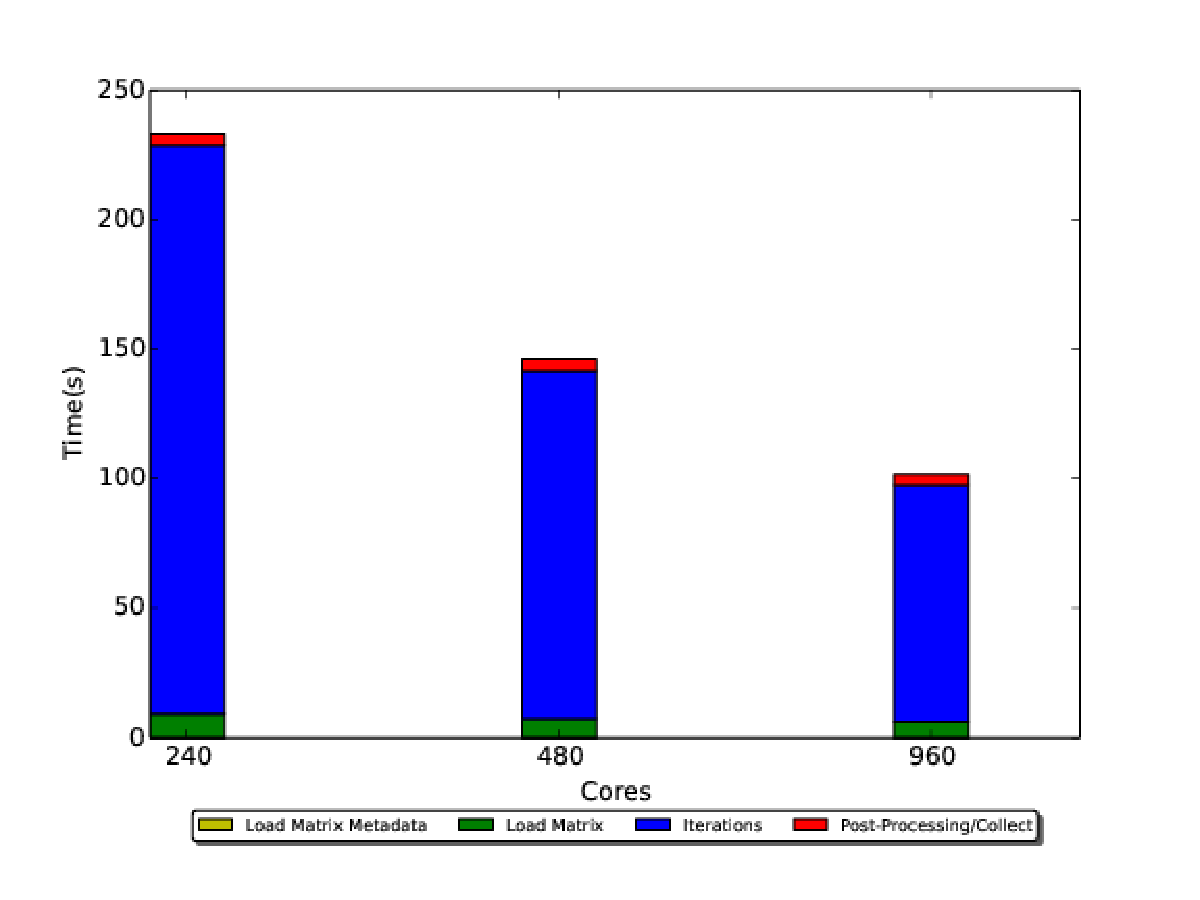
\includegraphics[scale=0.4]{images/CX_Strong_Scaling_Rank_32_Partitions_default.pdf}
    \end{centering}
    \caption{ Strong scaling for the 4 phases of CX on an XC40 for 100GB dataset at rank 32 and default partitioning as concurrency is increased.} 
    \end{figure} 


  \subsection{Comparison across Multiple Platforms}
    
    \begin{figure} [H]
    \begin{centering}
    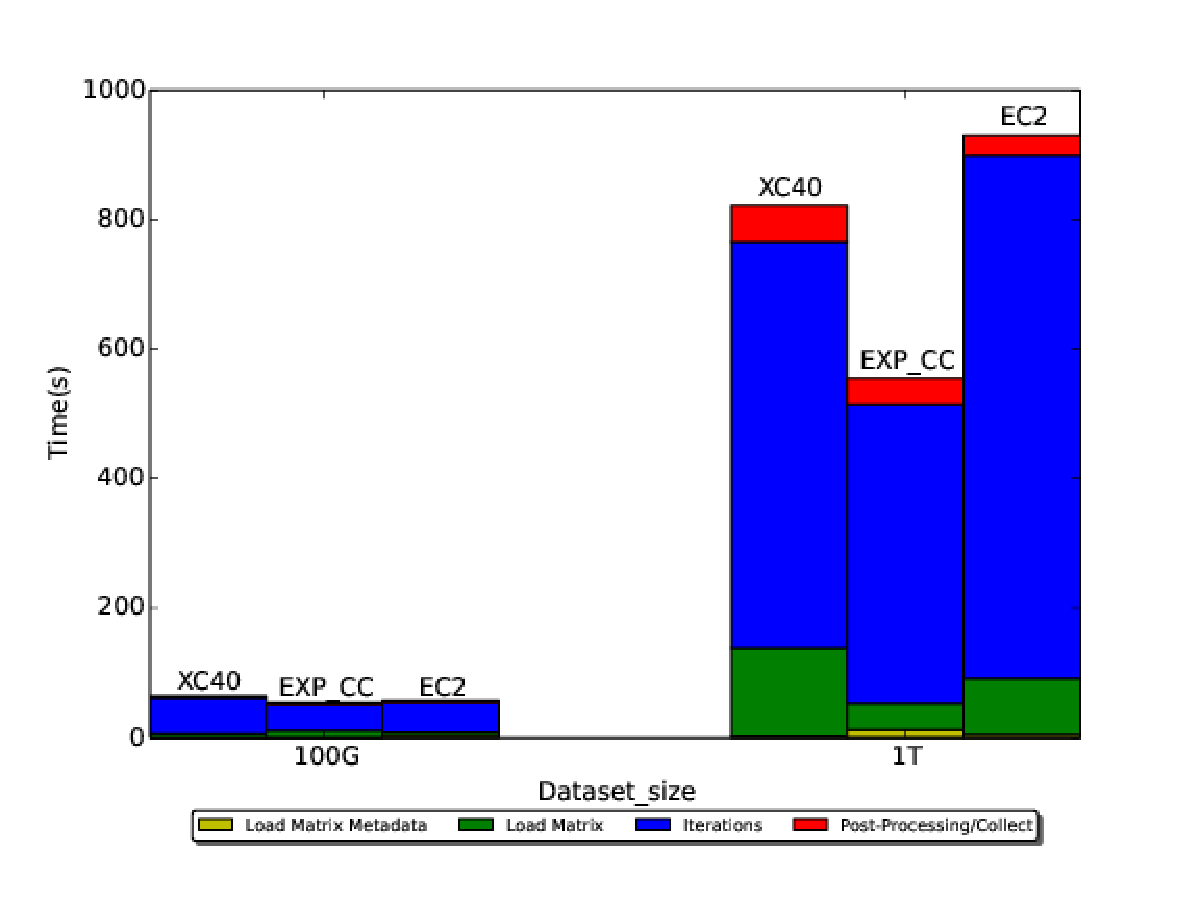
\includegraphics[scale=0.4]{images/CX_Size_Scaling_Rank_16_Partitions_default.pdf}
    \end{centering}
    \caption{ Run times for the various stages of computation for CX for two different dataset sizes for the three platforms using rank 16 and default partitioning for the given platform} 
    \label{fig:h2hrank16} 
    \end{figure}

    
      \begin{figure} [H]
    \begin{centering}
    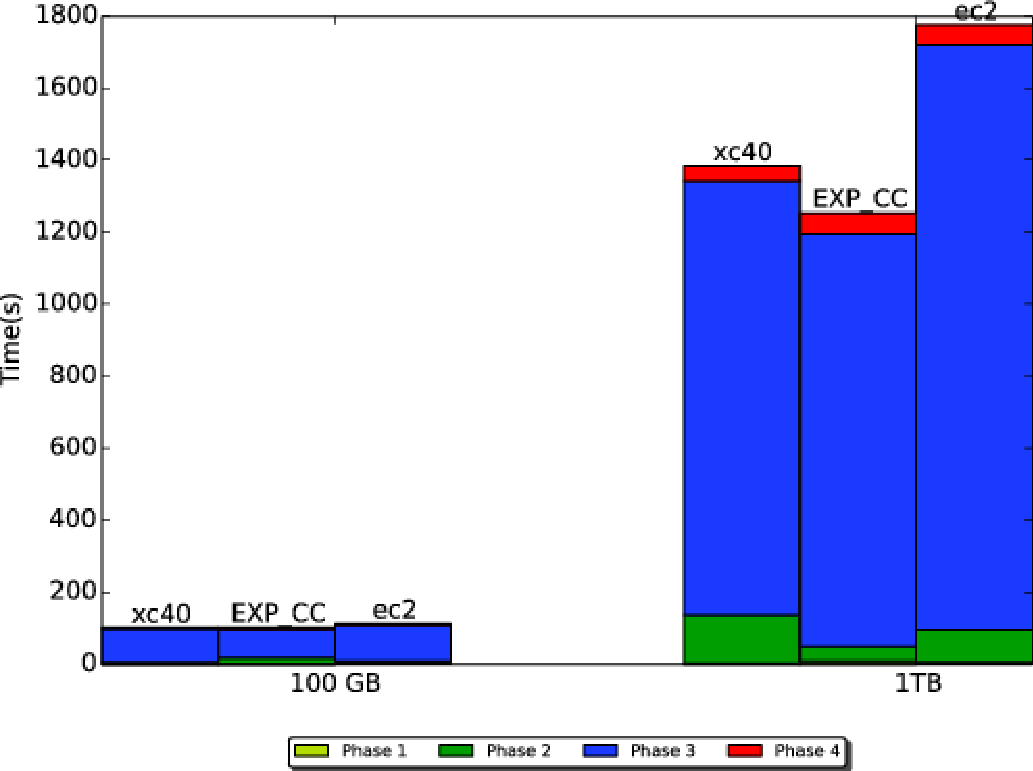
\includegraphics[scale=0.4]{images/CX_Size_Scaling_Rank_32_Partitions_default.pdf}
    \end{centering}
    \caption{ Run times for the various stages of computation for CX for two different dataset sizes for the three platforms using rank 32 and default partitioning for the given platform}
    \label{fig:h2hrank32} 
    \end{figure}
    
    \begin{table*}
    \begin{center}
    \begin{tabular}{| l | c | c | c | c | c | c | c |}
    \toprule
    \textbf{Platform} & \textbf{Rank} & \textbf{Total} & \textbf{Load} & \textbf{Time Per} & \textbf{Average} & \textbf{Average} & \textbf{Average} \\
                               & & \textbf{Runtime} & \textbf{Time} & \textbf{Iteration} & \textbf{Local} & \textbf{Aggregation} & \textbf{Network} \\
                               & & & & & \textbf{Task} & \textbf{Task} & \textbf{Wait} \\
    \midrule
    Amazon EC2 r3.8xlarge & 16 & 24.0 min & 1.53 min & 2.69 min & 4.4 sec & 27.1 sec & 21.7 sec \\
    \midrule
    Cray XC40 & 16 & 23.1 min& 2.32 min & 2.09 min &  3.5 sec & 6.8 sec & 1.1 sec \\
    \midrule
    Experimental Cray cluster & 16 & 15.2 min & 0.88 min & 1.54 min &  2.8 sec & 9.9 sec & 2.7 sec \\
    \midrule
    Amazon EC2 r3.8xlarge & 32 & 52.6 min& 1.57 min & 5.42 min &  8.7 sec & 60.1 sec & 48.7 sec \\
    \midrule
    Cray XC40 & 32 & 41.2 min & 2.28 min & 4.01 min &  7.5 sec & 25.0 sec & 15.4 sec \\
    \midrule
   Experimental Cray cluster & 32 & 35.8 min & 0.81 min & 3.82 min &  6.8 sec & 27.9 sec & 15.5 sec \\
   \bottomrule
    \end{tabular}
    \end{center}
    \caption{Total runtime for the 1 TB dataset, broken down into load time and per-iteration time. The per-iteration time is further broken down into the average time for each task of the local stage and each task of the aggregation stage.  We also show the average amount of time spent waiting for a network fetch, to illustrate the impact of the interconnect.}
    \label{tab:h2hres1TB}
    \end{table*}
    
Table~\ref{tab:h2hres1TB} shows the total runtime of CX for the 1 TB dataset on our three platforms.  The distributed Spark portion of the computation is also depicted visually in Figures~\ref{fig:h2hrank16} (rank 16) and~\ref{fig:h2hrank32} (rank 32).  All three platforms were able to successfully process the 1 TB dataset at rank 16 in under 25 minutes.  As the table and figures illustrate, most of the variation between the platforms occurred during the \texttt{MultiplyGramian} iterations.  Table~\ref{tab:hwspecs} shows the specifications of the three platforms. In this section, we explore how these difference relate to the performance of the matrix iterations.

  \begin{table*}
    \begin{center}
    \begin{tabular}{| l | c | c | c | c | c | c | c |}
    \toprule
    \textbf{Platform} & \textbf{Total Cores} & \textbf{Core Frequency} & \textbf{Interconnect} & \textbf{DRAM} & \textbf{SSDs} \\
    \midrule
    Amazon EC2 r3.8xlarge & 960 (32 per-node) & 2.5 GHz & 10 Gigabit Ethernet & 244 GiB & 2 x 320 GB \\
    \midrule
    Cray XC40 & 960 (32 per-node) & 2.3 GHz & Cray Aries\texttrademark & 252 GiB & None \\
    \midrule
    Experimental Cray cluster & 960 (24 per-node) & 2.5 GHz & Cray Aries\texttrademark & 126 GiB & 1 x 800 GB \\
    \bottomrule
    \end{tabular}
    \end{center}
    \caption{Specifications of the three hardware platforms used in these performance experiments.}
    \label{tab:hwspecs}
  \end{table*}

Spark divides each iteration into two stages.  The first \emph{local} stage computes each row's contribution, sums the local results (the rows computed by the same worker node), and records these locally-aggregated results.  The second \emph{aggregation} stage combines all of the workers' locally-aggregated results using a tree-structured reduction.  Most of the variation between platforms occurs during the aggregation phase, where data from remote worker nodes is fetched and combined.  In Spark, all inter-node data exchange occurs via \emph{shuffle operations}.  In a shuffle, workers with data to send write the data to their local scratch space.  Once all data has been written, workers with data to retrieve from remote nodes request that data from the sender's block manager, which in turns retrieves if from the senders local scratch space, and sends it over the interconnect to the receiving node.

Examining our three platforms, we notice two key hardware differences that impact shuffle operations.  First, both the EC2 nodes and the experimental Cray cluster nodes have fast SSD storage local to the compute nodes.  The Cray XC40, on the other hand, has no local block storage.  Thus it must emulate local storage with a remote Lustre filesystem.  The impacts of this can be somewhat mitigated, however, by leaving sufficient memory to store some of the scratch data in local RAM disk, and to locally cache some of the remote writes to Lustre.\footnote{This is an ideal usage of caching, since Spark assumes the scratch space is only locally accessible; thus we are guaranteed that the only node that reads a scratch file will be the same node that wrote it.}  Second, the Cray XC40 and the experimental Cray cluster both communicate over the HPC-optimized Cray Aries interconnect, while the EC2 nodes use 10 Gigabit Ethernet.  

We can see the impact of differing interconnect capabilities in the Average Network Wait column in Table~\ref{tab:h2hres1TB}.   These lower average network wait times explain why the two Cray platforms outperform the EC2 instance (with the experimental cluster achieving a speedup of roughly 1.5x over EC2).  The XC40 is still slightly slower than the experimental Cray platform, however, in particular at rank 16.  This can be understood by looking at the Maximum Aggregation Task and Maximum Network Wait columns.  \textbf{(NOTE: Verify that this is correct when Evan adds max data to Google Docs table, and add these to paper table.)}  Despite having lower average task and network wait times, the iteration time is actually higher because we have to synchronize after each iteration and wait for the slower tasks to complete.  These slow running tasks are indicative of data that was written to the remote Lustre filesystem and not locally cached (or subsequently evicted from the local cache).


  

  \subsection{Comparison of CX, PCA, RPCA quantitatively \textcolor{red}{Alex: please insert results here} }
    \begin{itemize}
      \item (for 100GB sized dataset on EC2)
      \item runtime vs. accuracy?
      \item show distinction b/w cx, pca
    \end{itemize}

  \subsection{Science plot for PCA, CX \textcolor{red}{Jiyan, Jey, Oliver, Ben: please insert results here}}
    \begin{itemize}
      \item PCA plot + science interpretation from Ben Bowen
      \item CX plot (spatial + ion dimensions) + science interpretation from Ben Bowen
    \end{itemize}

  \subsection{Lessons Learned}
  
  The differences in performance between the Cray\textregistered~XC40\textsuperscript{\tiny\texttrademark} system~\cite{alverson2012cray,craycascadesc12} and the experimental Cray cluster point to optimizations to Spark that could improve its performance on HPC-style architectures.  The two platforms have very similar configurations, with the primary difference being the lack of local persistent storage on the XC40 nodes.  As described in Section~\ref{sect:h2h}, this forces some of Spark's local scratch space to be allocated on the remote Lustre file system, rather than in local storage.  To mitigate this, and keep more of the scratch data local, we propose the following future investigations:
\begin{itemize}
\item Spark is currently inefficient in cleaning up its local scratch space.  In particular, shuffle data is not immediately cleaned up after a shuffle completes.  This makes fault recovery more efficient, but results in higher storage requirements for scratch space.  If clean up was more efficient, it would be more feasible to fit all of the scratch data in a local RAM disk and not rely on Lustre at all.
\item Spark does not currently allow you to configure primary and backup scratch directories.  Instead you list all scratch directories in a single list, and it distributes data in a round round fashion between them as long as space is available.  You can bias it towards one storage device (e.g., RAM disk vs. Lustre) by listing multiple directories on the preferred device.  Ideally, though, we would like to use a RAM disk (or other local storage) exclusively unless and until it fills, and only switch to Lustre directories if necessary.
\item Spark does not allow you to specify that a scratch directory is globally accessible.  Thus non-cached data is stored to the remote Lustre directory by the sender, and then later retrieved by the sender and sent to the receiver.  This wastes a step, since the receiver could easily fetch the data directly from Lustre (or any other global file system).
\item Alternatively, a push model of communication (as opposed to the current pull model) might be possible - however this would have implications for reliability and handling of very large data sets.\footnote{Storing the shuffle data to a large persistent block storage device, and only sending it as needed, allows Spark to easily shuffle more data than could fit in the remote buffers.  In a push-based model, extra logic and synchronization would be necessary to ensure that the remote buffers do not overflow.}
\end{itemize}



\section{Conclusions}
\label{sec:conclusion}

\begin{itemize}
\item Matrix factorizations are an important class of linear algebra problems. CX is a promising method for interpretable data analytics.
\item We have performed an in-depth analysis of performance of CX algorithm on a single node implementation, and a distributed node implementation utilizing Spark
\item We have performed a head-to-head study of our Spark implementation on state of the art HPC and data center platforms
\item We have applied the software to enable first-time science results on a massive 1TB sized mass spec imaging dataset
\end{itemize}


\bibliographystyle{abbrv}
\bibliography{heromsi}

\balancecolumns
\end{document}
